\documentclass[11pt,a4paper]{article}
\input{../../sablony/pripravy/priprava.sty}
\usepackage{tikz,pgfplots}
\pgfplotsset{compat=1.18}
\nastavPripravu{1. ročník}{Kvadratické rovnice a nerovnice}{114}{Kvadratické rovnice s absolutní hodnotou I}
\begin{document}
\blok{Kvadratické rovnice s absolutní hodnotou I}
Absolutní hodnota celého kvadratického výrazu: převrácení části grafu pod osou $x$.
\blok{Metoda a návaznost na graf}
\poznamka{U každého přechodu odmocněním platí $\sqrt{u^2}=|u|$, nikoli obecně $u$. Závěrečný graf ověřuje i platnost intervalových podmínek.}
\begin{itemize}
\item Základní graf $y=q(x)$ narýsuj z vrcholu a nulových bodů; při $y=|q(x)|$ zápornou část zrcadli podle osy $x$.
\item Rovnici $|q(x)|=c$ ($c\ge0$) řešíme jako $q(x)=c$ nebo $q(x)=-c$; vždy ověřujeme graf.
\end{itemize}
\blok{Tabulka: výraz uvnitř absolutní hodnoty}
\begin{center}\renewcommand{\arraystretch}{1.26}\small
\begin{tabular}{@{}lccc@{}}\toprule
$x$ & $(-\infty;-2)$ & $(-2;2)$ & $(2;+\infty)$\\\midrule
$x^2-4$ & $+$ & $-$ & $+$\\
$|x^2-4|$ & $+(x^2-4)$ & $-(x^2-4)$ & $+(x^2-4)$\\\midrule
Rovnice $|x^2-4|=3$ & $x^2-4=3$ & $-(x^2-4)=3$ & $x^2-4=3$\\\bottomrule
\end{tabular}
\end{center}
\poznamka{Kritické body $-2,2$ ověř zvlášť. Hranice nezapomínej ani při výpočtu přes dvě rovnice.}

\begin{center}
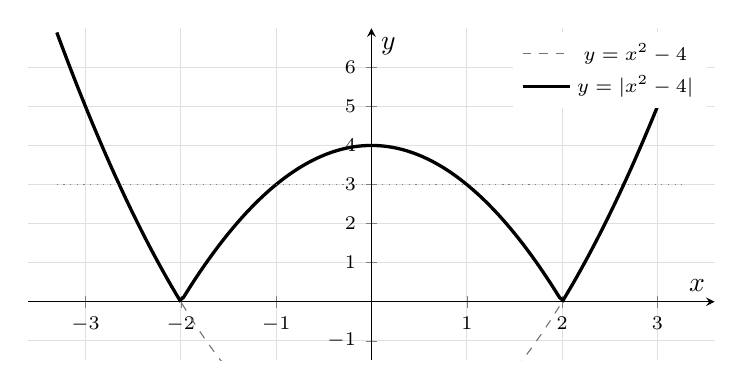
\begin{tikzpicture}
\begin{axis}[width=10.3cm,height=5.8cm,xmin=-3.6,xmax=3.6,ymin=-1.5,ymax=7,
axis lines=middle,grid=both,grid style={black!12},minor tick num=0, xlabel={$x$},ylabel={$y$},
xtick={-3,-2,-1,0,1,2,3},ytick={-1,0,1,2,3,4,5,6},
tick label style={font=\scriptsize},legend style={font=\scriptsize,draw=none,at={(.99,.99)},anchor=north east}]
\addplot[black!55,dashed,domain=-3.3:3.3,samples=180] {x^2-4};
\addlegendentry{$y=x^2-4$}
\addplot[black,very thick,domain=-3.3:3.3,samples=180] {abs(x^2-4)};
\addlegendentry{$y=|x^2-4|$}
\addplot[black!50,dotted,domain=-3.3:3.3] {3};
\end{axis}
\end{tikzpicture}
\end{center}
\poznamka{Přerušovaně původní parabola; plná čára po aplikaci absolutní hodnoty. Vodorovná hladina $y=3$ ukazuje čtyři průsečíky.}
\blok{Společně řešené příklady}
\begin{prikladReseniBox}[title={Příklad 1}]
$\left|x^{2} - 4\right|=3$
\tcblower
\[
\begin{aligned}
|f(x)|&=3\\[2pt]
f(x)&=3\quad\vee\quad f(x)=-3\\[2pt]
K_1&=\{- \sqrt{7};\sqrt{7}\}\\[2pt]
K_2&=\{-1;1\}\\[2pt]
K&=\{- \sqrt{7};-1;1;\sqrt{7}\}
\end{aligned}
\]
\end{prikladReseniBox}
\begin{prikladReseniBox}[title={Příklad 2}]
$\left|x^{2} - 4x + 3\right|=0$
\tcblower
\[
\begin{aligned}
|f(x)|&=0\\[2pt]
f(x)&=0\quad\vee\quad f(x)=-0\\[2pt]
K_1&=\{1;3\}\\[2pt]
K_2&=\{1;3\}\\[2pt]
K&=\{1;3\}
\end{aligned}
\]
\end{prikladReseniBox}
\begin{prikladReseniBox}[title={Příklad 3}]
$\left|x^{2} - 4x + 3\right|=2$
\tcblower
\[
\begin{aligned}
|f(x)|&=2\\[2pt]
f(x)&=2\quad\vee\quad f(x)=-2\\[2pt]
K_1&=\{2 - \sqrt{3};\sqrt{3} + 2\}\\[2pt]
K_2&=\varnothing\\[2pt]
K&=\{2 - \sqrt{3};\sqrt{3} + 2\}
\end{aligned}
\]
\end{prikladReseniBox}
\blok{Samostatné procvičování}
\begin{zadaniReseniBox}[title={Úloha 1}]
$\left|x^{2} - 9\right|=7$
\tcblower
\[
\begin{aligned}
|f(x)|&=7\\[2pt]
f(x)&=7\quad\vee\quad f(x)=-7\\[2pt]
K_1&=\{-4;4\}\\[2pt]
K_2&=\{- \sqrt{2};\sqrt{2}\}\\[2pt]
K&=\{-4;- \sqrt{2};\sqrt{2};4\}
\end{aligned}
\]
\end{zadaniReseniBox}
\begin{zadaniReseniBox}[title={Úloha 2}]
$\left|x^{2} - 2x - 3\right|=2$
\tcblower
\[
\begin{aligned}
|f(x)|&=2\\[2pt]
f(x)&=2\quad\vee\quad f(x)=-2\\[2pt]
K_1&=\{1 - \sqrt{6};1 + \sqrt{6}\}\\[2pt]
K_2&=\{1 - \sqrt{2};1 + \sqrt{2}\}\\[2pt]
K&=\{1 - \sqrt{6};1 - \sqrt{2};1 + \sqrt{2};1 + \sqrt{6}\}
\end{aligned}
\]
\end{zadaniReseniBox}
\blok{Volitelná grafická rezerva}
Porovnejte náčrty $y=|x^2-4|$ a $y=x^2-4$: které části zůstávají a které se převrátí?
\blok{Domácí úkol}
\begin{zadaniReseniBox}[title={Domácí příprava}]
\begin{enumerate}[label=\alph*),itemsep=2pt]
\item $\left|x^{2} - 4\right|=0$
\item $\left|x^{2} - 9\right|=5$
\item $\left|x^{2} - 4x + 3\right|=1$
\item $\left|x^{2} - 4x + 3\right|=4$
\item $\left|x^{2} - 1\right|=2$
\item $\left|x^{2} + 2x - 3\right|=3$
\end{enumerate}
\tcblower
\begin{enumerate}[label=\alph*),itemsep=2pt]
\item
\[\begin{aligned}
|f(x)|&=0\\[2pt]
f(x)&=0\quad\vee\quad f(x)=-0\\[2pt]
K_1&=\{-2;2\}\\[2pt]
K_2&=\{-2;2\}\\[2pt]
K&=\{-2;2\}
\end{aligned}\]
\item
\[\begin{aligned}
|f(x)|&=5\\[2pt]
f(x)&=5\quad\vee\quad f(x)=-5\\[2pt]
K_1&=\{- \sqrt{14};\sqrt{14}\}\\[2pt]
K_2&=\{-2;2\}\\[2pt]
K&=\{- \sqrt{14};-2;2;\sqrt{14}\}
\end{aligned}\]
\item
\[\begin{aligned}
|f(x)|&=1\\[2pt]
f(x)&=1\quad\vee\quad f(x)=-1\\[2pt]
K_1&=\{2 - \sqrt{2};\sqrt{2} + 2\}\\[2pt]
K_2&=\{2\}\\[2pt]
K&=\{2 - \sqrt{2};2;\sqrt{2} + 2\}
\end{aligned}\]
\item
\[\begin{aligned}
|f(x)|&=4\\[2pt]
f(x)&=4\quad\vee\quad f(x)=-4\\[2pt]
K_1&=\{2 - \sqrt{5};2 + \sqrt{5}\}\\[2pt]
K_2&=\varnothing\\[2pt]
K&=\{2 - \sqrt{5};2 + \sqrt{5}\}
\end{aligned}\]
\item
\[\begin{aligned}
|f(x)|&=2\\[2pt]
f(x)&=2\quad\vee\quad f(x)=-2\\[2pt]
K_1&=\{- \sqrt{3};\sqrt{3}\}\\[2pt]
K_2&=\varnothing\\[2pt]
K&=\{- \sqrt{3};\sqrt{3}\}
\end{aligned}\]
\item
\[\begin{aligned}
|f(x)|&=3\\[2pt]
f(x)&=3\quad\vee\quad f(x)=-3\\[2pt]
K_1&=\{- \sqrt{7} - 1;-1 + \sqrt{7}\}\\[2pt]
K_2&=\{-2;0\}\\[2pt]
K&=\{- \sqrt{7} - 1;-2;0;-1 + \sqrt{7}\}
\end{aligned}\]
\end{enumerate}
\end{zadaniReseniBox}
\poznamka{Orientační čas: úvod 5 min, společné příklady 18 min, samostatně 15 min, kontrola a shrnutí 7 min. Rezerva je dobrovolná. Číselné parametry modelových aplikací nejsou skutečně naměřená data.}
\end{document}
